\section{Executing Commands} \label{subsec_IExecutionInteractorObject}

An exciting implementation that facilitates a high degree of cohesion while maintaining
low coupling is the utilization of the \code{koks_iexecutioninteractor_2023} interface
\parencite{koks_iexecutioninteractor_2023}. This interface allows for the execution of
various derived types responsible for specific tasks, such as executing Handlers,
Harvesters, and Rejuvenators \parencites{koks_expandentitieshandlerinteractor_2023,
koks_regionharvesterinteractor_2023, koks_regionrejuvenatorinteractor_2023}. The
implementation promotes decoupling by adhering to both \gls{ocp} and \gls{lsp}.

\begin{figure}[H]
    \centering
    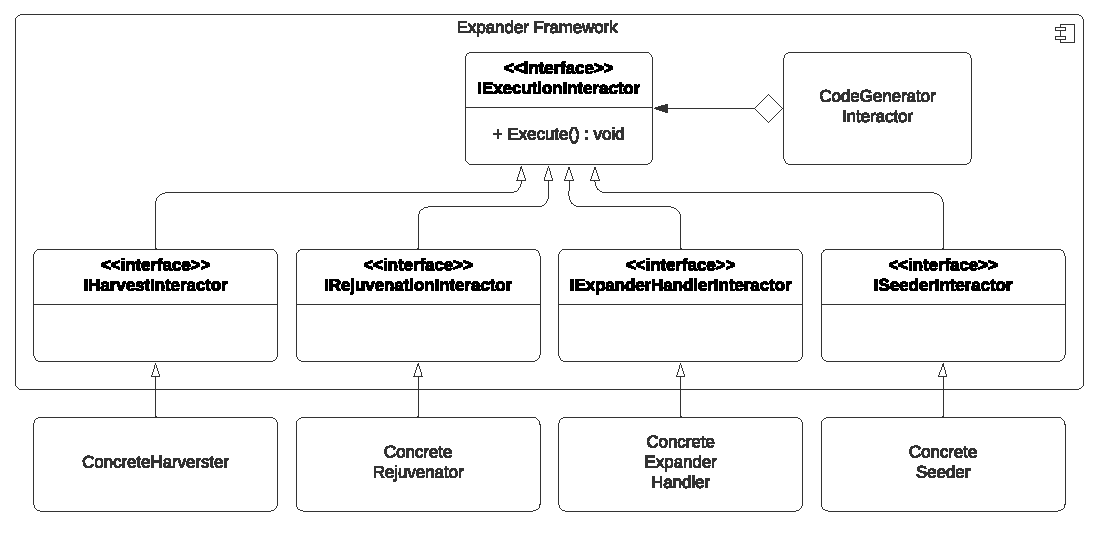
\includegraphics[width=1\textwidth]{figures/command_pattern.pdf}
    \caption[Low coupling with \code{koks_iexecutioninteractor_2023}]{Low coupling with \code{koks_iexecutioninteractor_2023}}
    \label{fig_iexecutioninteractor}
  \end{figure}


Figure \ref{fig_iexecutioninteractor} illustrates that the required interfaces are placed
in the Domain layer of the Expander Framework. In contrast, the concrete classes also can
be implemented as part of the internal scope of the Clean Architecture Expander
\parencite{koks_migrationharvesterinteractor_2023}. Code listing
\fullref{list_expandentitieshandlerinteractor} illustrates an implementation example of
this interface. Finally, the code listing \fullref{list_CodeGeneratorInteractor}
illustrates the aggregation of the execution, which allows for a graceful cohesion of the
execution Tasks \parencite{koks_codegeneratorinteractor_2023}.
